%!TEX root = ../Main.tex

\chapter{研究二}\label{ch-name2}
\section{引言}
xxx

\section{xxx}\label{sec-x x}
x描述:
\begin{equation}\begin{aligned}
	I &= M_{\text{idexy}}(\Theta_{\text{idxity}}) \\
	A &= M_{\text{xar}}(I, \Theta_{\text{xtar}}) \\
	B &= M_{\text{xxhy}}(I, \Theta_{\text{bixphy}}) \\
	\{T_1, T_2, \ldots, T_n\} &= M_{\text{twx}}(I, C, \Theta_{\text{txt}})
\end{aligned}\end{equation}
其中,\(\Theta_{\text{idexy}}\), \(\Theta_{\text{axr}}\), \(\Theta_{\text{bixhy}}\), 和 \(\Theta_{\text{txt}}\) 分别代表各模型的x征。


xxxx

\begin{table}[htbp]\footnotesize
	\centering
	
	\begin{threeparttable}[b]
		\bicaption{DPxx细信息}{Detailed infxx framework}
		\label{sec-llms}
		\begin{tabular}{@{}lllllll@{}}
			\hline%\toprule
			\rowcolor{gray!15}
			\textbf{机构} & \textbf{x} & \textbf{x} & \textbf{x} &  \textbf{x} & \textbf{x} & \textbf{x} \\ \hline%\midrule
			x           & Gxx-2\cite{journalkey}               & x-xl\tnote{1}  & 1.x              & Dec-x       & x & x\cite{journalkey}                   \\
			x      & Mistral\cite{conferencekey}              & x-7B-v0.1\tnote{2}  & x            & x-x       & N/A & x                   \\
			x      & LLaMA 2\cite{conferencekey}              & 
			x-2-x-x-hf\tnote{3}  & 7B           & Enc-Dec       & N/A & Mix                   \\
			x           & x-Neo\cite{conferencekey}              & x-x-2.7B\tnote{4}  & 2.x            & x-only       & N/A & Pile\cite{journalkey}                   \\
			x & x\cite{journalkey} & x-x\tnote{5} & 6B & Dec-only & GLM & Mix \\ 
			\hline%\bottomrule
		\end{tabular}%	
		
		\begin{tablenotes}
			\item[1] https://hxx-xl
			\item[2] https://xxistral-x
			\item[3] https://huxhf
			\item[4] https://huxx
			\item[5] https://hxnxx
		\end{tablenotes}
	\end{threeparttable}
\end{table}


\begin{table}[ht]\footnotesize
	\bicaption{TI-xx的性能表现}{TI-SAxataset}
	\label{tab:imxxtion}
	\centering
	\begin{threeparttable}[b]
		\begin{tabular}{>{\columncolor{gray!15}}m{4cm}||cc||ccc}
			\hline
			& \multicolumn{2}{c||}{\cellcolor{gray!15}\textbf{x}} & \multicolumn{3}{c}{\cellcolor{gray!15}\textbf{x(高亲和力)}} \\
			\cline{2-6}
			\multirowcell{-2}{\textbf{x}} & \cellcolor{gray!15}x$\downarrow$ & \cellcolor{gray!15}R-x(\%)$\uparrow$ &  \cellcolor{gray!15}x$\downarrow$ & \cellcolor{gray!15}R-x(\%)$\uparrow$ & \cellcolor{gray!15}P-x$\downarrow$\\
			\hline
			\cellcolor{white}\textbf{TI-x-x} & \underline{86.x} & \underline{92.17}  & \underline{93.74}  & \underline{89.13}  & \underline{26.x} \\
			\hline
			\cellcolor{white}w/o x w x & 138.54 & 75.16  & 146.37 & 71.15 & 47.51 \\
			\cellcolor{white}w/o x w FULL & 117.72 & 77.03  & 122.01 &  72.57 & 47.03  \\
			\hline
			\cellcolor{white}w/o x & \textbf{78.32} & \textbf{95.89}  & \textbf{83.46} & \textbf{93.42} &  44.39 \\
			\cellcolor{white}w/o x & 138x.69 & 74.98  & 139.60 & 71.42 &  \textbf{20.73} \\
			\hline
			\cellcolor{white}w/o x & 106.74 & 83.31  & 117.67 & 79.93 & 36.01 \\
			\cellcolor{white}w/o x & 88.06 & 90.72  & 97.32 & 87.05 & 29.10 \\
			\hline
		\end{tabular}
	\begin{tablenotes}
		\item[*] x,因此衡量P-x
	\end{tablenotes}
	\end{threeparttable}
\end{table}



\subsection{案例分析}

\subsubsection{x}

本文xx像(如图\ref{fig:avatar gen case study}(\subref{fig_female})和图\ref{fig:avatar gen case study}(\subref{fig_male}))和指xx性比较(如图\ref{fig:avatar gen case study}(\subref{fig_female_agreeable})和图\ref{fig:avatar gen case study}(\subref{fig_female_agreeable}))。
\vspace{12pt}
\begin{figure*}[!htbp]
	\centering
	\subfloat[]{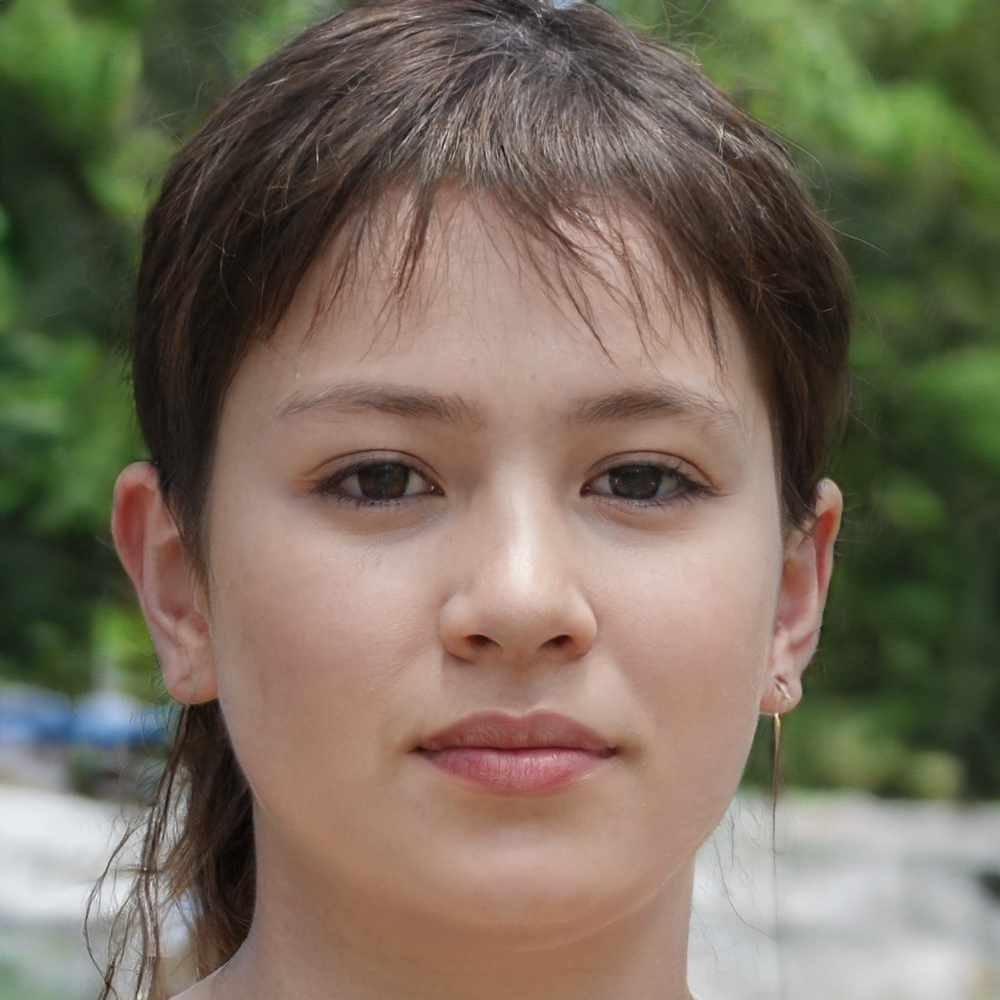
\includegraphics[width=1.8in]{Figures/sample-14}% 1.5
		\label{fig_female}}
	\hfil
	%	\hspace*{\fill}
	\subfloat[]{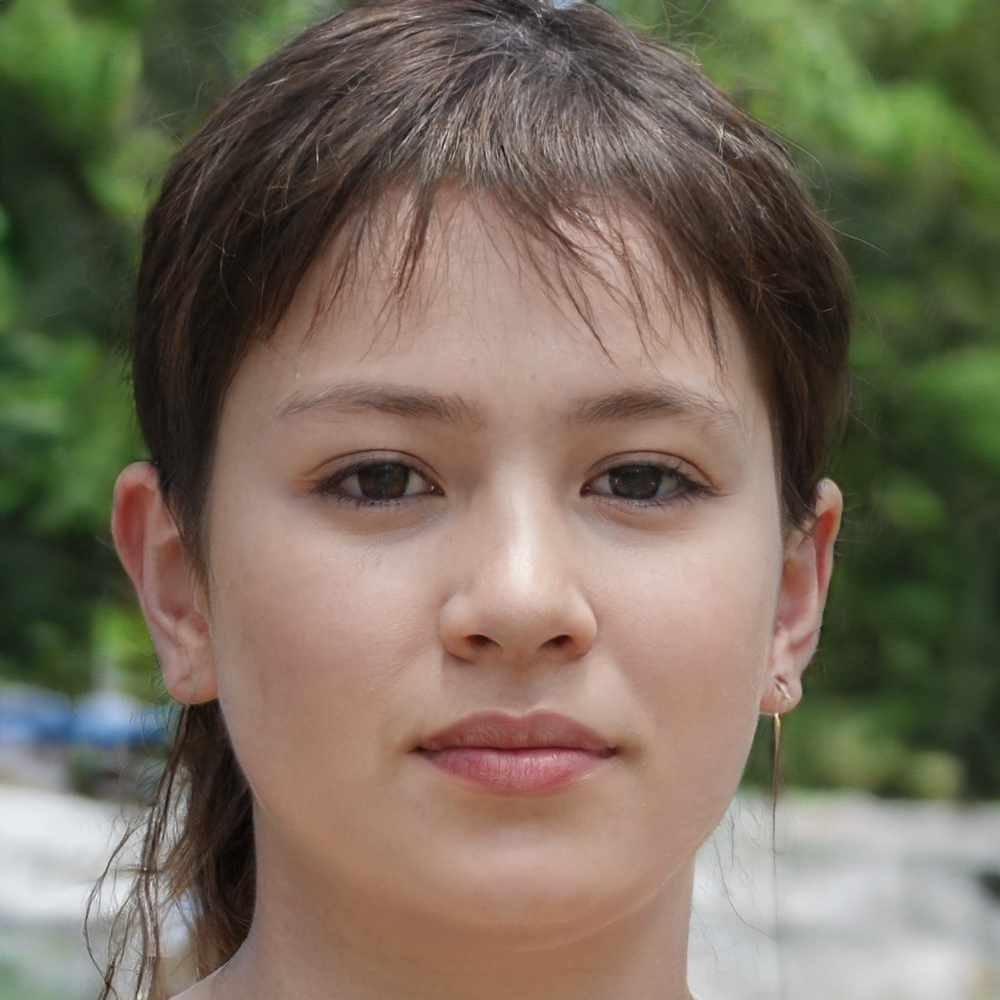
\includegraphics[width=1.8in]{Figures/sample-12}% 1.5
		\label{fig_female_agreeable}}
	\\ \vspace*{12pt}
	\subfloat[]{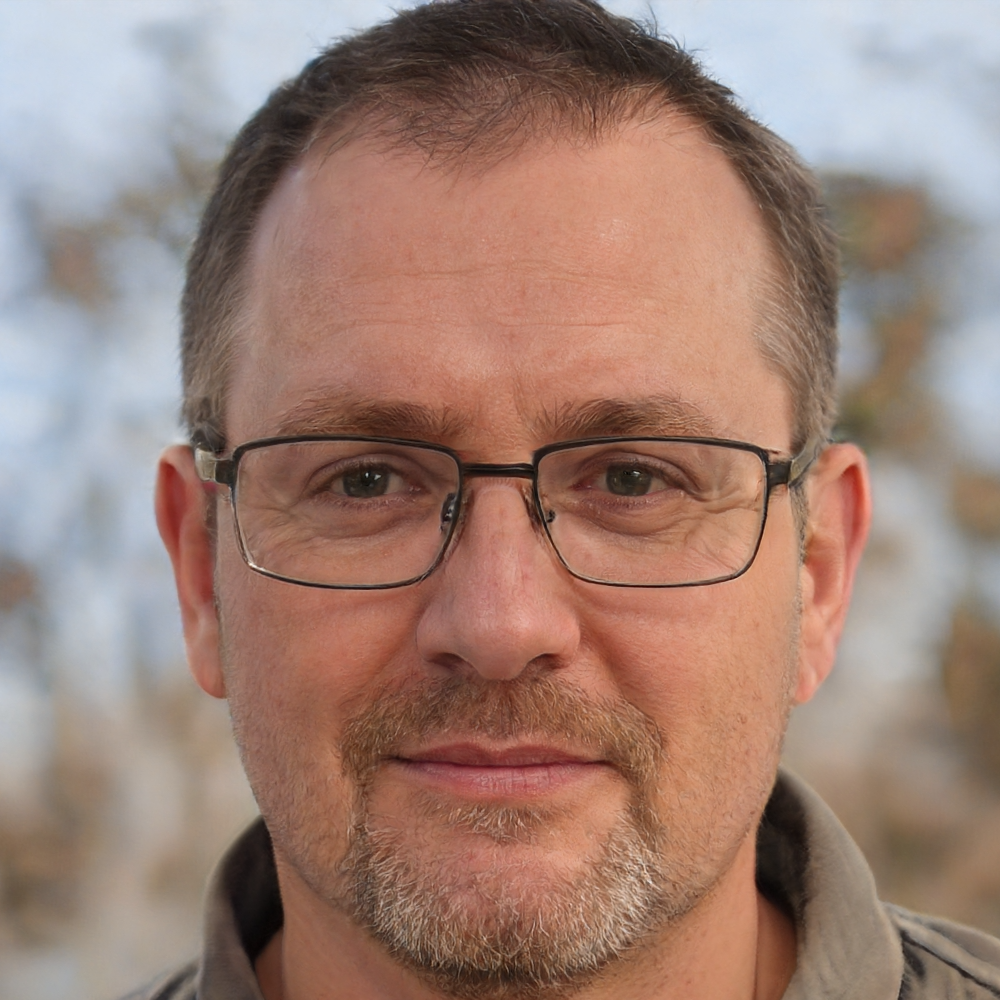
\includegraphics[width=1.8in]{Figures/sample-35}% 1.5
		\label{fig_male}}
	\hfil
	\subfloat[]{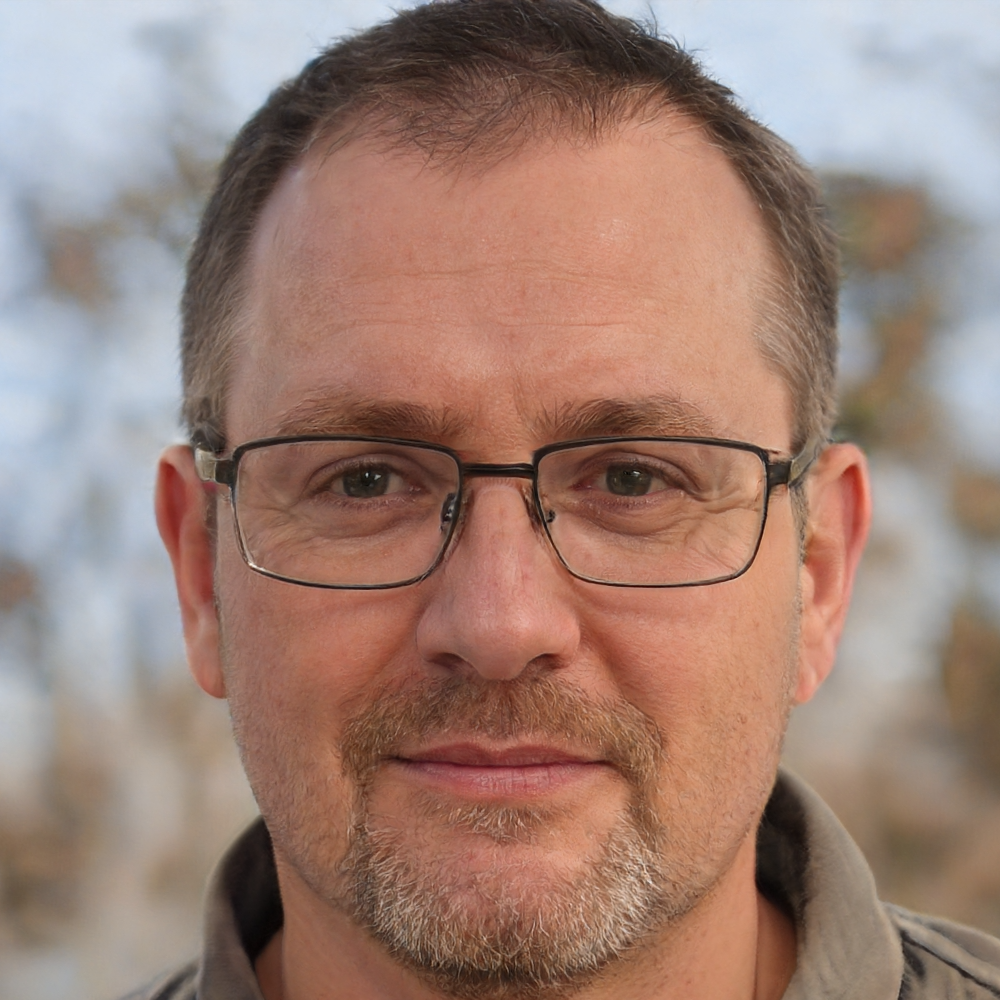
\includegraphics[width=1.8in]{Figures/sample-39}% 1.5
		\label{fig_male_agreeable}}
	\bicaption{不xx例}{Sampxxities}
	\label{fig:avatar gen case study}
\end{figure*}

x

\section{本章小结}
xx



